\documentclass[tikz,border=2pt]{standalone}
\usepackage{amsmath}
\usepackage{amssymb}
\usepackage{xcolor}

\definecolor{journalink}{HTML}{1F1C18}
\definecolor{journalmuted}{HTML}{8A7F72}
\definecolor{journalaccent}{HTML}{9C2D2D}

\newcommand{\sssig}{\scriptscriptstyle}

\begin{document}
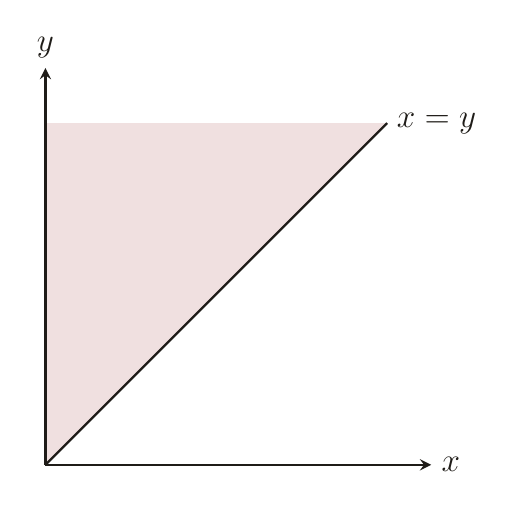
\begin{tikzpicture}[x=1.4cm, y=1.4cm, >=stealth,
                    every node/.style={journalink, font=\large}]

  %% 聯合值域 y > x > 0 所對應的區域: 直線 x = y 的左上方
  \fill[journalaccent, fill opacity=0.15]
    (0,0) -- (3.1,3.1) -- (0,3.1) -- cycle;

  %% 邊界 x = y
  \draw[journalink, line width=0.8pt] (0,0) -- (3.1,3.1);
  \node[journalink, right] at (3.1,3.1) {$x=y$};

  %% 座標軸
  \draw[journalink, line width=0.8pt, ->] (0,0) -- (3.5,0) node[right] {$x$};
  \draw[journalink, line width=0.8pt, ->] (0,0) -- (0,3.6) node[above] {$y$};

\end{tikzpicture}
\end{document}
